\chapter{相关基础研究}
\label{chapter:background}

本章将介绍普通和加密重复数据删除、可信执行环境(TEE)等本文利用的基础知识,以及加密重复数据删除系统中存在的性能瓶颈和安全性隐患。

\section{重复数据删除}
\label{sec:background-deduplication}

本文专注于基于数据块的重复数据删除,它以称为数据块的小型数据单元为粒度运行。基于数据块的重复数据删除比基于文件的重复数据删除更精细,因此通常具有更高的存储效率(节省更多的存储空间)。基于数据块的重复数据删除有以下两种基本的数据块分块方法:

\begin{itemize}[leftmargin=0em]
    \item \textbf{固定大小的数据分块(Fixed-size chunking)},通常将文件划分为固定长度的数据块,具有简单快速的特点,但文件中小范围修改(例如:增加或删除1字节内容)将从修改位置开始影响后续所有数据块的内容(即,边界漂移问题\citing{muthitacharoen2001low}),将严重降低重复数据删除的空间节省效果。
    \item \textbf{可变大小的数据分块(Variable-size chunking)},也称为内容定义的数据块分块\textit{(Content-defined chunking, CDC)}。通常采用内容相关的方式指定数据块的边界(例如,通过Rabin指纹\citing{rabin1981fingerprinting}在特定内容模式出现时进行分块)。因此,在文件发生小范围修改时,产生的大多数数据块仍可保持不变,使得重复数据删除系统存储效率得到保障。
\end{itemize}

在多数备份系统工作负载\citing{zhu2008avoiding,lillibridge2009sparse}下,可变大小的数据分块方案通常可以获得更优的存储效率,但在某些特定工作负载(例如,VM备份数据集\citing{jin2009effectiveness})下,固定大小的数据分块方案却更加有效。本文的工作可兼容固定大小和可变大小的数据分块方法产生的数据块。

\begin{figure}[!htb]
    \small
    \centering
    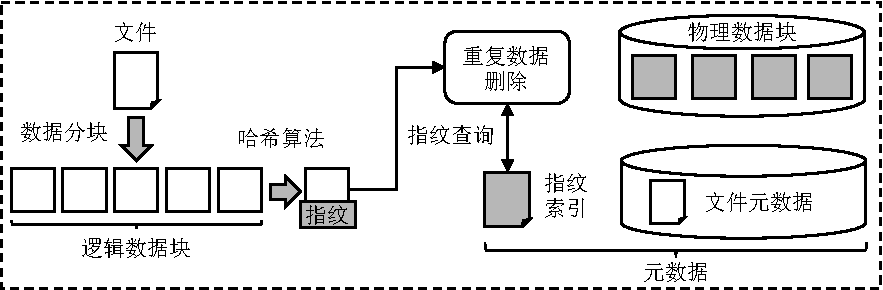
\includegraphics[width=\textwidth]{pic/background/chunk-based-dedup-arch.pdf}
    \caption{基于数据块的重复数据删除的工作流程概览}
    \label{fig:chunk-based-dedup-flow}
\end{figure}

图\ref{fig:chunk-based-dedup-flow}总结了基于数据块的重复数据删除工作流程。具体地,重复数据删除系统首先通过数据分块过程将客户端的文件(例如,备份文件)分割为逻辑数据块,根据每一个逻辑数据块的内容,使用哈希算法计算得到其对应的唯一标签(又称为指纹)。如果两个数据块具有相同的指纹,则认为两个数据块内容相同(不同逻辑数据块计算得到相同指纹的概率可忽略不计\citing{black2006compare});若两个逻辑数据块指纹不一致,则认为两逻辑数据块不同。重复数据删除系统仅存储相同逻辑数据块的唯一副本(称为物理数据块),并且每个相同的逻辑数据块仅通过一个空间开销较小的索引指向相同的物理数据块。此外,基于数据块的重复数据删除系统记录文件所拥有的所有逻辑数据块的信息作为该文件的元数据,用于文件读取、删除等操作。

重复数据删除技术根据重复数据删除操作发生的位置可分为源端重复数据删除及目标端重复数据删除\citing{IDC2010Data}:

\begin{itemize}[leftmargin=0em]
    \item \textbf{源端重复数据删除(Source-based Deduplication)}由客户端计算目标数据块的哈希值,并由服务端检查该哈希值是否存在于索引表中。如果哈希值存在(即服务端已有目标数据块的副本),则通知客户端无需传输目标数据块。
    \item \textbf{目标端重复数据删除(Target-based Deduplication)}强制客户端传输所有密文数据块,并在服务端对所有收到的密文数据块进行重复数据删除。
\end{itemize}

源端重复数据删除技术可有效节省网络流量资源,可显著降低云服务商提供存储服务的成本,但泄露了“其他客户端是否已经存储相应密文数据块”的侧信道信息(参见\S\ref{subsubsec:intro-problem-security});目标端重复数据删除具有更高的隐私保护能力,但产生大量网络资源浪费,并显著增加了服务端计算开销。本文关注网络资源开销较小的源端重复数据删除技术,并通过TEE技术解决其存在的性能和安全性问题。

\section{安全重复数据删除}
\label{sec:background-enc-deduplication}

加密重复数据删除解决了外包环境(例如,云存储)中的数据块机密性保障问题,同时保持了重复数据删除的有效性。出于安全因素考虑,用户希望将自己的数据加密后再进行外包存储,以确保个人数据隐私性。传统对称加密算法算法为每个客户端或每个逻辑数据块分配独立的加密密钥,使得来自不同(或相同)客户端的相同的逻辑数据块被加密为不同的密文数据块,服务器无法感知这些密文数据块所对应的明文数据块内容是否一致,使得针对外包数据的重复数据删除完全失效。

\begin{figure}[!htb]
    \small
    \centering
    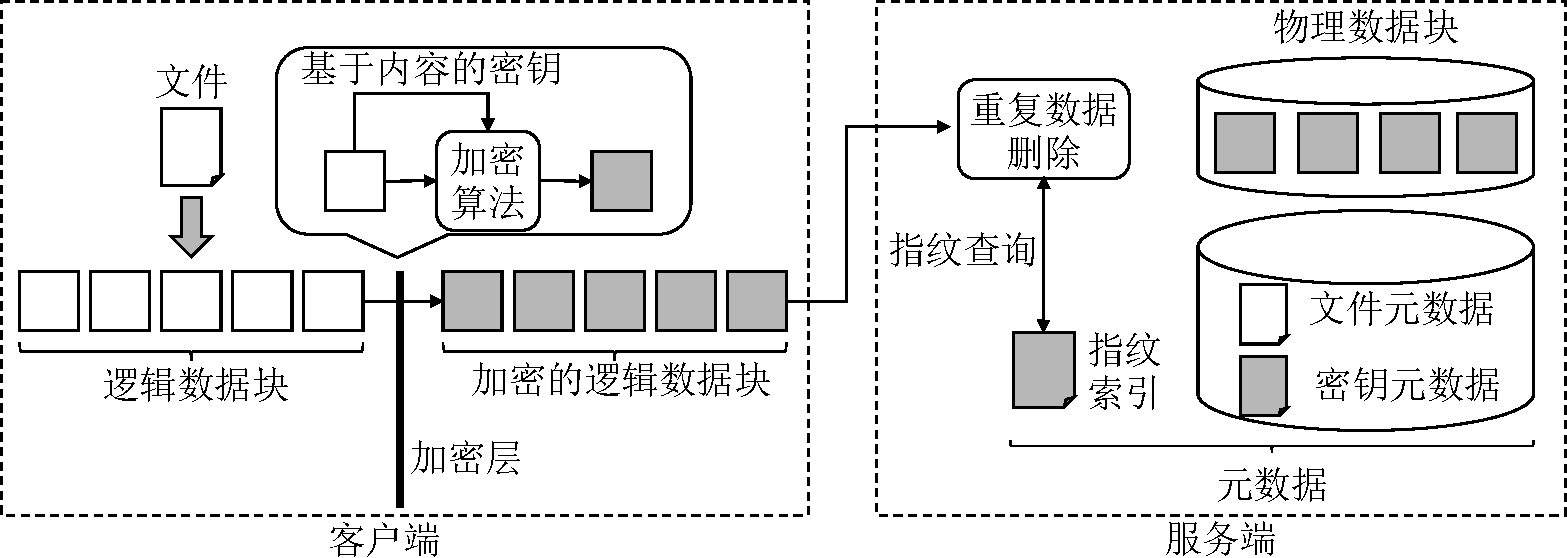
\includegraphics[width=\textwidth]{pic/background/chunk-based-enc-dedup-arch.pdf}
    \caption{基于数据块的加密重复数据删除的工作流程概览}
    \label{fig:chunk-based-enc-dedup-flow}
\end{figure}

如图~\ref{fig:chunk-based-enc-dedup-flow}所示,基于内容的密钥生成方法给加密重复数据删除提供了新的处理思路。最基本的基于内容的密钥生成方法的实例化是基于明文数据的内容(例如,基于重复数据删除中的逻辑数据块)导出其对称加密密钥,并使用该密钥加密明文数据以形成对应的密文数据(例如,加密的逻辑数据块)。因此,使用基于内容的密钥生成方法为任意逻辑数据块产生对称加密密钥可以确保将相同的明文数据块加密为相同的密文数据块。最后,存储系统从每个密文数据块中导出其对应的指纹并执行重复数据删除。相较于普通重复数据删除,加密重复数据删除需额外保存用户文件所包含数据块的密钥元数据,并由各个客户端进行加密以防止服务端取得相应数据块的明文内容。

\subsection{数据块加密技术}
\label{subsec:background-encrypted-deduplication-key}

消息锁加密\textit{(Message-Locked Encryption, MLE)}\citing{bellare2013MLE}将基于内容的密钥生成方案等加密原语形式化用于加密重复数据删除。它指出了如何从明文数据块的内容导出相应的对称加密密钥(称为消息锁加密密钥,简称为MLE密钥)。以最广泛使用的消息锁加密技术:收敛加密\textit{(Convergent Encryption, CE)}\citing{douceur2002reclaiming}为例,CE使用明文数据块的安全哈希作为MLE密钥,使得相同的明文数据块可被加密为相同的密文数据块,从而令重复数据删除技术在密文数据块之上仍然可行。除此之外,基于CE的消息锁加密方案还包括:

\begin{enumerate}[leftmargin=0em]
    \item \textbf{哈希收敛加密(Hash Convergent Encryption, HCE)}\citing{douceur2002reclaiming}与CE具有相同的MLE密钥产生规则,但基于明文哈希值计算指纹用于重复数据删除。作为对比的,CE使用密文的指纹进行重复数据删除检查。
    \item \textbf{随机收敛加密(Random Convergent Encryption, RCE)}\citing{douceur2002reclaiming}使用随机密钥加密明文以产生非确定的密文,但基于明文的哈希值进行重复数据删除检查。
    \item \textbf{收敛扩散(Convergent Dispersa, CD)}\citing{li2016cdstore}使用明文哈希值作为秘密共享(Secret Sharing)的输入种子,并对产生的多个秘密共享分别计算哈希并进行重复数据删除,在兼容重复数据删除的基础上提高了密文存储的可靠性。
\end{enumerate}

然而,CE容易受到\textbf{离线暴力破解攻击}的威胁。这是由于CE的MLE密钥(即明文数据块的哈希)可以自由产生。具体来说,攻击者通过枚举所有可能的明文数据块的MLE密钥来从目标密文数据块(其加密密钥未知)推断输入的明文数据块,以检查是存在某个明文数据块被加密到目标密文数据块。

服务器辅助消息锁加密\textit{(Server-aided MLE)}\citing{bellare2013DupLESS}是最先进的加密原语,可增强加密重复数据删除对离线暴力攻击的安全性。它为消息锁加密中的MLE密钥生成步骤部署了一个专用的\textbf{密钥服务器(Key server)}。为了加密明文数据块,客户端首先将明文数据块的指纹发送到密钥服务器,密钥服务器通过指纹和密钥服务器维护的\textbf{全局秘密(Global secret)}返回MLE密钥。如果全局秘密是安全的,则攻击者无法发起离线暴力攻击;如果全局秘密被泄露,则其安全性会降低到原始消息锁加密的安全性。服务器辅助消息锁加密建立在如下两种安全机制之上:

\begin{itemize}[leftmargin=0em]
    \item \textbf{遗忘伪随机函数(Oblivious pseudorandom function, OPRF)}\citing{naor2004Number}是一种包含服务端和客户端的安全多方计算协议。其中,服务端持有密钥$k$,客户端持有输入$x$,协议双方联合计算函数$f_k(x)$,并确保最终仅由客户端得到所计算的目标函数值。OPRF协议采用双盲方式执行,即计算过程中可确保服务端无法获得客户端输入且客户端无法获得服务端密钥。
    \item \textbf{速率限制(Rate-limiting)}\citing{bellare2013DupLESS}阻止特定操作频率超出某些限制。在大型系统中,速率限制通常用于保护底层服务和资源。
\end{itemize}

基于遗忘伪随机函数,密钥服务器可依据客户端发送明文数据块的“盲化指纹”,进而基于盲指纹和全局秘密产生对应数据块的“盲化密钥”,阻止了密钥服务器了解明文数据块信息;并使得客户端可在不了解密钥服务器所拥有的全局秘密的条件下获得目标明文数据块的MLE密钥。对来自客户端的密钥生成请求进行速率限制,进一步防止恶意客户端向密钥服务器发出海量密钥生成请求以获得目标MLE密钥,限制了攻击者暴力破解攻击的速度。

\subsection{数据所有权证明技术}
\label{subsec:background-encrypted-deduplication-pow}

为了节省宝贵的网络带宽资源,现有加密重复数据删除系统普遍采用源端重复数据删除,以便在客户端删除重复数据块,而无需上传到服务端(\S\ref{sec:background-deduplication})。但是,源端重复数据删除导致“目标数据块是否已在服务端存储”的侧信道信息,使得某些客户端存在恶意时,源端重复数据删除很容易受到侧信道攻击\textit{(Side-channel attack)}\citing{harnik2010side,halevi11}的影响。

一种典型的侧信道攻击被称为\textbf{伪造所有权攻击}:恶意客户端未授权访问其他客户端存储的数据块\citing{harnik2010side,mulazzani11}。具体来说,由于服务端仅能基于收到的数据块哈希值判断客户端是否拥有对应的数据块,攻击者可使用任意目标密文数据块的指纹来说服服务端其是该目标数据块的所有者,进而获得该数据块的完全访问权限(\S\ref{subsec:intro-background});另一种侧信道攻击被称为\textbf{推测内容攻击}:恶意客户端将目标密文数据块指纹发送到服务端以检查该数据块是否存在(例如,目标密文数据块对应于某个可能的密码\citing{harnik2010side}),以此识别来自其他客户端的敏感信息(\S\ref{subsubsec:intro-problem-security})。

现有防御机制尚无法在执行源端重复数据删除且不大量增加额外网络带宽资源开销的前提是防御推测内容攻击。而为了防止伪造所有权攻击,源端加密重复数据删除增加了所有权证明\textit{(Proof-of-ownership, PoW)}机制\citing{halevi11},要求客户端额外向服务端提交目标密文数据块的所有权证明(Proof),且仅在所有权证明成功的条件下进行重复数据删除。所有权证明机制可使得服务端只针对客户端真实拥有(即具有完整访问权限)的密文数据块执行重复数据删除,避免了攻击者非法访问其他客户端已在云服务端存储的内容。现有基于Merkle树的所有权证明机制(称为POW-MT)\citing{xu2013weak}使用纠删码对数据块进行编码,随后在纠删码编码结果的基础上建立Merkle树用于所有权证明。而另一种基于通用哈希函数\textit{(Universal hash)}的所有权证明机制(称为POW-UH)\citing{halevi2011proofs} 相较于基于Merkle树的所有权证明机制拥有更高的效率,但降低了安全性假设。

本文关注网络和服务端计算资源开销较小的源端重复数据删除技术,并通过TEE技术解决其存在的密钥生成和所有权证明效率问题,以及易受到推测内容攻击的安全性问题。

\section{可信执行环境(TEE)}
\label{sec:background-tee}

可信执行环境(Trusted Execution Environment, TEE)\citing{tee}是一种在计算平台上由软硬件协同构建的安全区域。其设计目标是确保安全区域中的程序按照预期执行,保证程序初始状态和运行时的机密性、完整性。基于GlobalPlatform组织\citing{GP}对TEE的标准规范,各个软硬件厂商结合自身基础架构构建的TEE存在显著差异,但各类TEE均具有以下主要特性:

\begin{itemize}[leftmargin=0em]
    \item \textbf{隔离性}:
          TEE将其中的目标程序、数据等与外部环境隔离,使得TEE外软硬件均无法获得其内部的机密信息。最早的隔离机制出现于Intel 80286处理器,其提供了两种具有不同安全权限的CPU运行模式,并在之后的X86架构处理器上衍生出各类具有不同权限的特权界别。近年来,Intel提出了安全区域范围更小的可信执行环境SGX(Intel Software Guard Extensions)\citing{sgx};同样的,ARM提出了TrustZone技术通过时分复用的方式为CPU提供了安全世界\textit{(Secure World)}与非安全世界\textit{(Normal World)}的隔离。
    \item \textbf{软硬协同性}:
          标准定义下允许厂商单独使用软件或硬件机制实现TEE,但在实际开发的产品中,厂商往往选择结合软件及硬件的方案设计TEE。
    \item \textbf{富表达性}:
          与传统安全芯片或纯软件的密码学隐私保护机制相比,TEE支持更丰富的上层应用。软件开发者仅需根据业务需求合理划分程序的隐私与非隐私部分,且TEE不会对其中运行的程序的算法逻辑、程序语言等方面进行额外限制。即,TEE内部是图灵完备的。同时,TEE内部的数据无需进行复杂的密态运算,使得其中的应用可支持更多复杂的算法。
\end{itemize}

\subsection{Intel SGX}
\label{subsec:background-tee-sgx}

\begin{figure}[!htb]
    \small
    \centering
    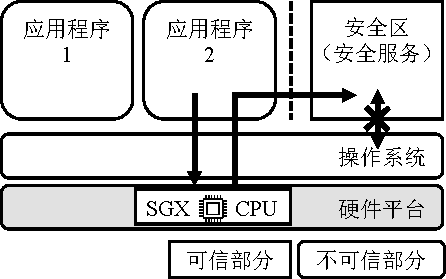
\includegraphics[width=0.5\textwidth]{pic/background/sgx-example.pdf}
    \caption{Intel SGX框架}
    \label{fig:sgx-arch}
\end{figure}

Intel Software Guard Extensions (Intel SGX)\citing{sgx,sgx2},是一组内置于现代Intel CPU中用于增强应用程序代码和数据安全性的扩展指令。开发者可利用SGX技术将应用程序的安全操作封装在称为“安全区\textit{(Enclave)}”的硬件保护环境中,保障用户关键代码和数据的机密性和完整性。Intel SGX最关键的优势在于将应用程序以外的软件栈如操作系统(OS)和基本输入输出系统(BIOS)都排除在了可信计算基(Trusted Computing Base, TCB)之外,一旦程序和数据在安全区之中,即便是操作系统也无法影响安全区内的代码和数据,安全区的安全边界只包含CPU和它本身(如图\ref{fig:sgx-arch}所示)。Intel SGX具有隔离、证明和密封三项主要安全功能。

\textbf{隔离(Isolation)}:安全区代码和数据被放置在被称为\textit{Enclave page cache (EPC)}的硬件内存保护区域中,该内存区域使用内存加密引擎(MEE)进行加密,以防止泄露任何内存数据到本安全区之外。EPC以大小为4\,KiB的页面为基本单位管理安全区内存,任意安全区内应用程序最多可占用96\,MiB内存空间\citing{harnik2018SGX}。当安全区内存使用超过上限时,须将未使用的内存页面加密并逐出到未受保护的主存,并在将逐出的页面加载回安全区内存时解密并验证完整性,导致巨大的分页开销\citing{arnautov2016SCONE,dinhngoc2019Everything}。

此外,SGX为安全区和未受保护的内存之间的交互提供了两个接口,应用程序可以通过安全区内部调用(ECalls)进入安全区以执行安全区内部函数,并且在ECall中,程序可通过安全区外部调用(OCalls)暂时退出安全区并调用不受保护的内存中的不受信任的函数。但安全区内部调用和外部调用会产生大量的CPU上下文切换开销\citing{harnik2018SGX},严重影响SGX应用程序性能。

\textbf{认证(Attestation)}:SGX安全区支持本地认证\textit{(Local Attestation)}和远程认证\textit{(Remote Attestation)},以确保安全区内运行的程序未被修改。特别的,在远程认证过程(参见\citing{SGX-RA}提供的端到端远程认证示例)中,远程实体(例如,服务端)需要联系Intel运营的证明服务来检查目标安全区提供的安全区相关信息的完整性和正确性。随后,远程实体通过将其收到的安全区信息与目标安全区中预期的可信信息进行比较来验证目标安全区是否未被修改。然而,由于远程认证需要Intel服务器的支持,远程认证过程通常导致较高且不可控的时间开销。

\textbf{密封(Sealing)}: SGX安全区通过密封在安全区内容需要在安全区外持久化存储时进行保护。它使用目标安全区专用的密封密钥(Sealing key)在数据被移出安全区之前进行加密。密封密钥可以从安全区测量哈希(\textit{Measurement hash},即安全区内容的SHA-256哈希)或安全区的创建者提供的签名身份派生。基于前者产生的密封密钥仅有目标安全区本身可以导出,而基于后者产生的密封密钥可有同一开发者创建的各个不同的安全区导出。因此,仅有相应的安全区才能获得正确的密封密钥并解密密封数据。

\subsection{ARM TrustZone}
\label{subsec:background-tee-tz}

ARM TrustZone\citing{trustzone}是ARM公司为Cortex-A微架构\citing{cortex-a}设计的一种TEE解决方案,并在最新的指令集架构中扩展至Cortex-M微架构\citing{cortex-m}。TrustZone技术通过对原有ARM处理器硬件架构进行修改,将处理器划分为两个具有不同安全权限的运行环境(两运行环境通过时分复用共享处理器资源):安全世界(Secure World)和非安全世界(Normal World),并防止运行于非安全世界的软件直接访问安全世界资源。

如图~\ref{fig:ARM-TZ-base}(a)所示,ARM引入了一种称为监视模式的处理器模式,该模式负责在世界过渡时保留处理器状态,两个世界可以通过称为安全监视器调用(Secure Monitor Call, SMC)的特权指令进入监视模式并实现彼此切换。

\begin{figure}[!htb]
    \small
    \centering
    \begin{tabular}{@{}c@{}c@{}c}
        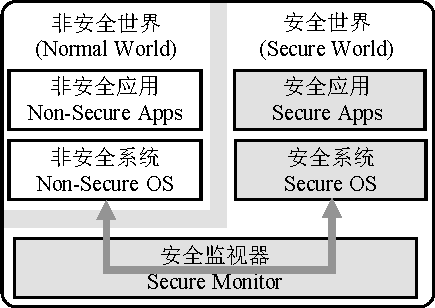
\includegraphics[width=0.49\textwidth]{pic/background/ARM-TZ-A.pdf} &
        \hspace{5pt}
        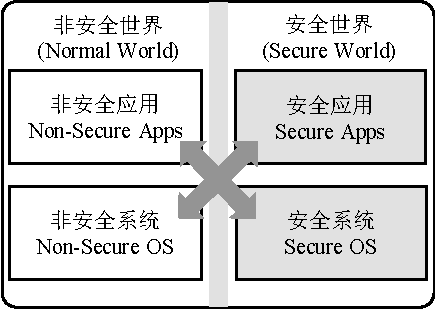
\includegraphics[width=0.49\textwidth]{pic/background/ARM-TZ-M.pdf}   \\
        \mbox{\small (a) Cortex-A微架构中的TrustZone}                       &
        \mbox{\small (b) Cortex-M微架构中的TrustZone}                         \\
    \end{tabular}
    \caption{ARM TrustZone技术}
    \label{fig:ARM-TZ-base}
\end{figure}

与Cortex-A相同的是,Cortex-M依旧将处理器运行状态划分为安全世界和非安全世界,并阻止运行于非安全世界的软件直接访问安全资源。不同的是,Cortex-M针对更快的上下文切换和低功耗应用进行了优化。具体来说,Cortex-M中世界之间的划分是基于内存映射的,并且转换是在异常处理代码中自动发生的(如图~\ref{fig:ARM-TZ-base}(b)所示)。这意味着,当从安全内存运行代码时,处理器处于安全世界,而当从非安全内存运行代码时,处理器处于非安全世界。Cortex-M中的TrustZone技术排除了监视模式,也不需要任何安全的监视软件,这大大减少了安全世界与非安全世界的切换延迟,使得世界之间的转换为更高效。总体而言,基于TrustZone技术,处理器厂商、开发者可以搭建一个可信执行环境(TEE),并在TEE内运行可信执行环境操作系统\textit{TEE OS}(例如,高通QSEE\citing{qsee}、OP-TEE\citing{op-tee})。

\section{本章小结}

本章介绍了普通与加密重复数据删除,现有加密重复数据删除中数据块加密技术和数据所有权证明技术导致的性能问题,以及可信执行环境的相关内容。
